A continuación explicaremos los resultados obtenidos en cada una de las redes.

Como mencionamos, en la red doméstica realizamos la recopilación de los datos con y sin intervención. Pudimos ver que al desconectar y conectar los dispositivos a la red, se generaban alrededor de 20 a 30 paquetes ARP. De modo que encontramos diferencias entre ambas experimentaciones. Los gráficos siguientes muestran un aspecto de ambas corridas: cada nodo del grafo es un nodo de la red, y los ejes dirigidos apuntan de un nodo v a otro w si hubo algun mensaje tal que el pSrc es igual al IP de v y el pDst es igual al IP de w. Además los nodos varían en tama\~no de acuerdo a la cantidad de paquetes a ARP que emitieron, siendo los más grandes los nodos que emitieron más mensajes ARP:

\begin{figure}[!h]
	\begin{center}
		  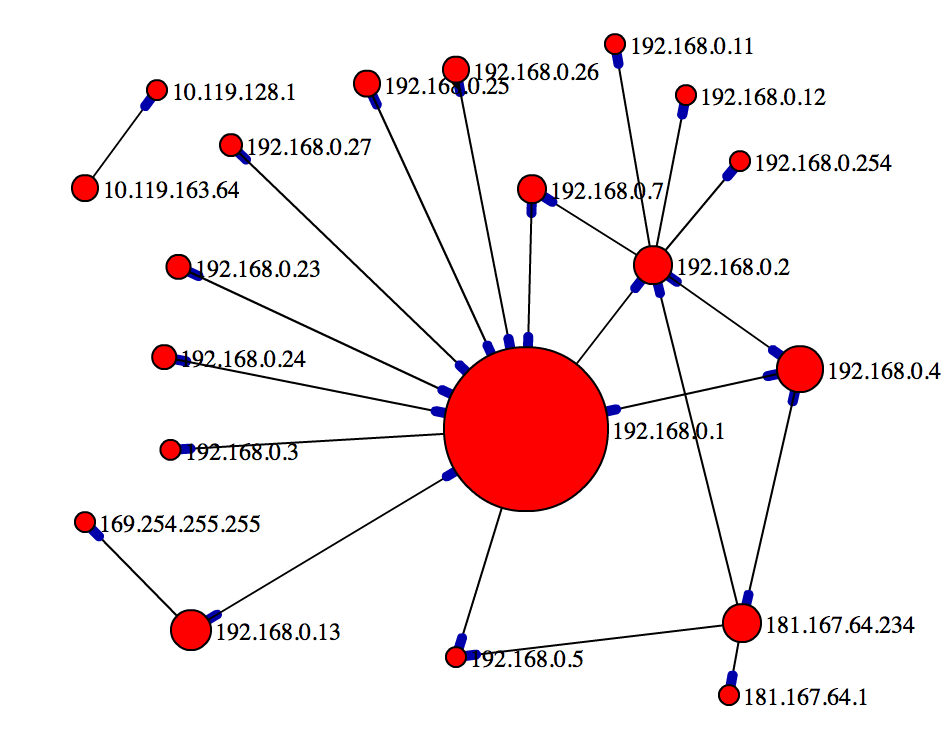
\includegraphics[scale=0.4]{Graficos/grafico_1.png}
		  \caption{Red doméstica, experimento 1}
		  \label{fig:contra1}
	\end{center}
\end{figure}

\begin{figure}[!h]
	\begin{center}
		  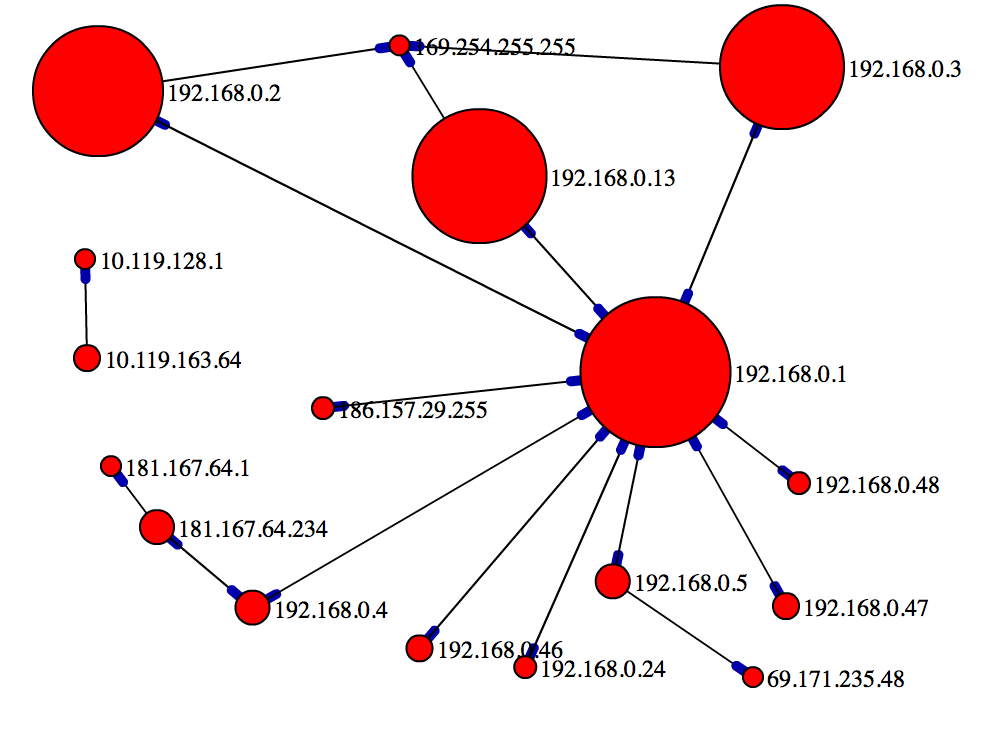
\includegraphics[scale=0.4]{Graficos/grafico_2.png}
		  \caption{Red doméstica, experimento 2}
		  \label{fig:contra1}
	\end{center}
\end{figure}

En ambos gráficos se ve claramente cuál es el gateway de la red, en este caso 192.168.0.1, ya que todos los nodos se comunican con ese nodo. Además es el nodo que envía mas mensajes ARP, lo cual se ve por su tama\~no mayor a los demás. 

En la segunda experimentación, a pesar de que el gateway continúa siendo el nodo de mayor tama\~no, hay otros que son casi iguales a él, lo que indica que enviaron casi la misma cantidad de paquetes ARP. Analizando los paquetes enviados por esos nodos, vimos que muchos son enviados al router, pero que gran parte de esos paquetes son enviados a la direccion 169.254.255.255. Segun la documentacion de Apple[1](los dispositivos son en su mayoria de Apple) esos paquetes son causados porque los dispositivos no encuentran el servidor DHCP, esto sucede cuando se los desconecta ya que pierden la ruta al servidor y entonces cuando se los vuelve a conectar, entonces envían mensajes ARP a esa direccion. 

Tambien vimos que hay paquetes que son enviados desde y hacia la direccion 181.167.64.234, la cual es la dirección pública que tiene el router a internet. Vemos que intercambia mensajes con  181.167.64.1 y creemos que es un router del ISP. Hay otros mensajes enviados desde esa dirección hacia la red local, pero desconocemos la razón de estos mensajes ARP. 

Tampoco sabemos la procedencia de otras IPs que parecieran ser dispositivos de la red(192.168.0.x) pero que no pudimos identificar y hay otras IPs que parecieran estar fuera de la red como 10.119.163.64 y 10.119.128.1, pero aún así están enviando mensajes ARP con broadcast en la red local. Realizando una búsqueda en internet no pudimos encontrar información sobre esas IPs.

Realizamos otra experimentación en una red pública(Starbucks). Dado que la red es pública, no teníamos conocimiento alguno de los dispositivos en ella y estos se desconectaban y conectaban aleatoriamente. Obtuvimos los siguientes resultados:

\begin{figure}[!h]
	\begin{center}
		  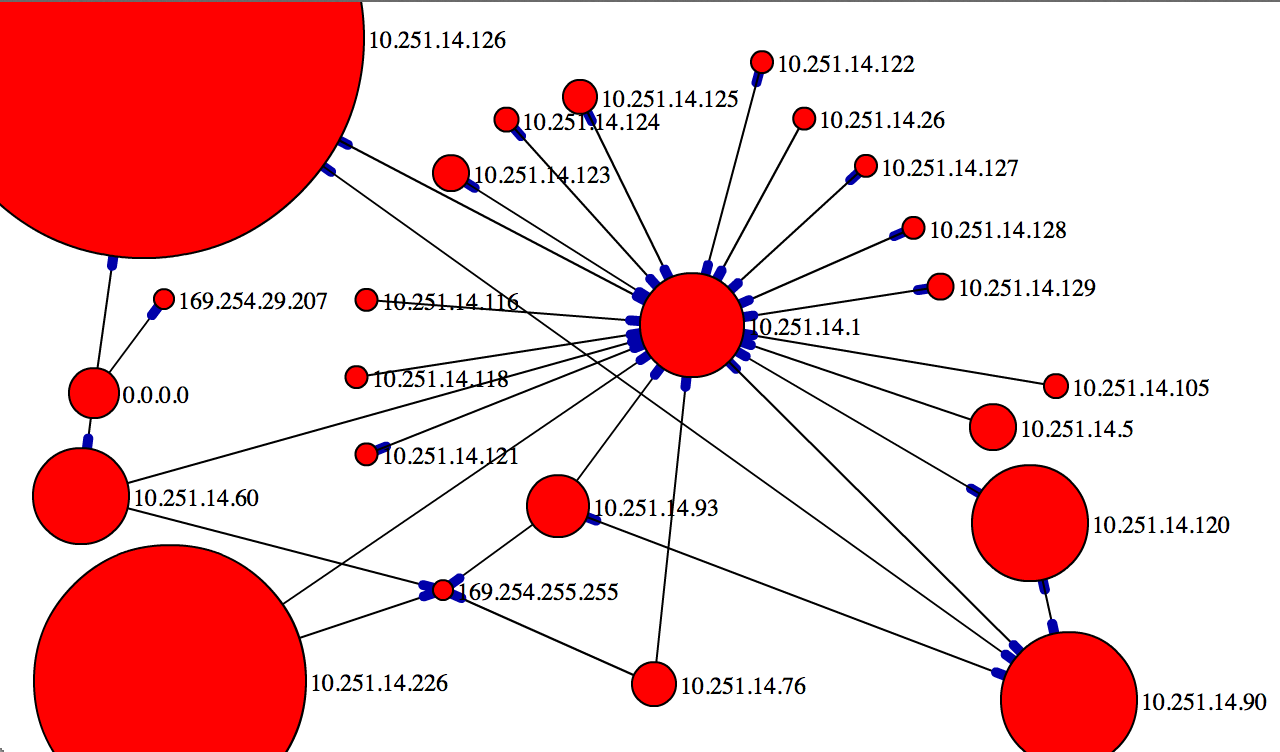
\includegraphics[scale=0.4]{Graficos/grafico_3.png}
		  \caption{Red de Starbucks}
		  \label{fig:contra1}
	\end{center}
\end{figure}

Nuevamente es sencillo identificar cuál es el gateway en la red: 10.251.14.1. Lo que nos llamó mucho la atención es la existencia de dos nodos(los más grandes) que emitían paquetes ARP casi de forma constante. El mayor de ellos mandaba muchos de sus paquetes a la direccion 0.0.0.0. Suponemos que ese funcionamiento es particular de la red de Starbucks que usa FibertelZone como una capa intermedia para conectarse.

Por último, observemos los resultados obtenidos en la red del centro médico. Al igual que la red de Starbucks, no conocíamos cómo se encontraba estructurada la red. Estos fueron los resultados:

\begin{figure}[!h]
	\begin{center}
		  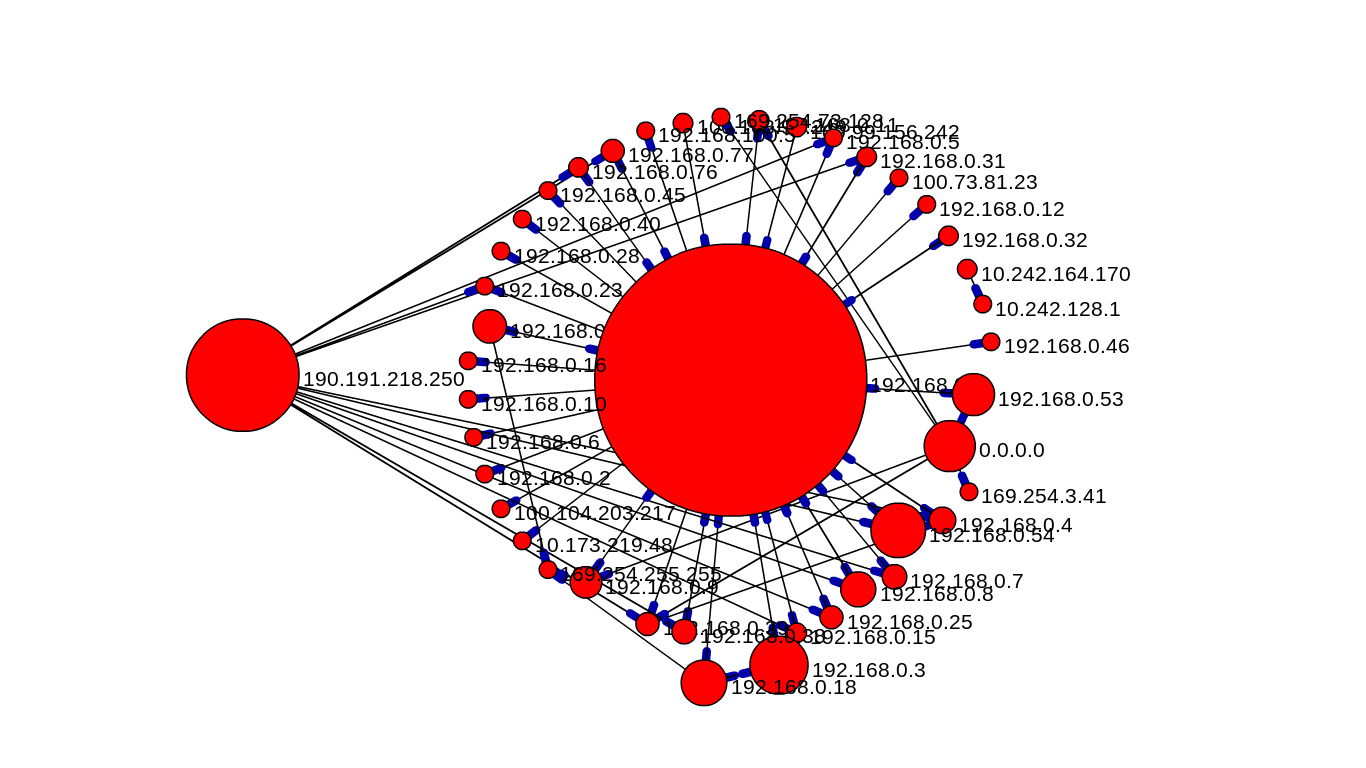
\includegraphics[scale=0.4]{Graficos/grafico_4.png}
		  \caption{Red de un centro médico}
		  \label{fig:contra1}
	\end{center}
\end{figure}

Claramente el gateway de la red es: 192.168.0.1. También notamos la presencia de un nodo (190.191.218.250) que envía paquetes a varios dispositivos de la red local y al gateway cuya dirección ip nos hace deducir que no pertenece a la LAN. Buscando información en internet averiguamos que se trata de la dirección del ISP que pertenece al grupo Clarín.	


